\chapter{原理与方法}

引言中提到的与内核相关的弱震相在实际资料中都十分稀少,但它们对内核物理性质的研究却非常重要,
就目前来说甚至是不能被其他方法所替代的,如自由震荡\citep{DZIEWONSKI1971};存在分辨率不高
的缺陷;目前比较流行的噪声干涉方法最初用于提取地球表层面波信号\citep{Snieder2004}, 最近
也有关于内核相关的体波提取的发现\citep{Lin2013,Lin2013b}, 但都还处于初步的研究阶段。所以
相比而言,较为“传统”的地震台阵方法对于这些内核弱震相的提取还是很重要的。

地震台阵方法兴起于上世纪六十年代,当时主要是出于核爆监测的需要,它的发展为现代地震学注入了新的
活力。假设远震地震体波可以看作平面波,通过台阵的叠加,极大提高了地震信号的信噪比,而且地震台阵
同时兼具慢度和方位角的分辨率,使得过去一些不易甚至不能在单台上观测到的震相被地震学家观测到,其中
就包括前临界PKiKP\citep{Schlittenhardt1996}、PKIIKP\citep{Niu2008}相位。新的台阵叠加
技术也不断涌现\citep{Rost2002},从最开始的简单叠加、线性叠加,到各种非线性叠加技术,即增强连续
的一致的信号,削弱不连续的随机的噪声,显著地放大了所需的弱相位。现在比较常用的非线性叠加技术有
加权相位叠加(PWS)\citep{Schimmel1997},N次根叠加\citep{Muirhead1976}等。

\section{叠加与FK分析的关系}

不论是什么叠加方法,在其数据处理过程中都对信号进行了延迟然后在求和的操作,只是最终求和的时候使用的
加权方式不同而已。这种延迟求和操作在地震学上成为Beamforming,而从本质来说这种操作和频率波数域谱
分析具有紧密的联系。下面参照\citep{hinich1981}的推导过程来说明叠加与FK分析的本质联系。

首先考虑最简单的情况: 一个由M个台站组成的线状台阵和一个单色简谐平面波。$\theta_{0}$表示波的传播方向与台站轴线的夹角,$c$为
波的视速度,$A$为波的振幅。则在不考虑噪声的情况下,第$k$个台站所接收到的信号可以表示为

\begin{equation}
s(t,x_k) = A exp[i \omega_{0} (t-x_k cos\theta_{0}/c)]
\end{equation}

在一个角度$\theta$叠加的Beam信号为

\begin{equation}
B(t,\theta) = \sum_{k=1}^{M} s(t+\tau_{k},x_k)
\end{equation}

其中第$k$个台站接收到的信号延迟时间$\tau_{k} = x_k cos\theta /c$。 因为波数分量可以写成
$\kappa = ((\omega /c) cos \theta$, 因而由上面两式可以得到 

\begin{eqnarray}
B(t,\theta) & = & A exp(i \omega_{0} t) \sum_{k=1}^{M} exp[i (\kappa - \kappa_{0})] \\
 & = &  s(t,x_k) exp(i\kappa x_k)
\end{eqnarray}

可以看出线性beamforming实际上就是计算了台阵接收到信号的空间域傅立叶变换。在实际的数据处理中
通常要根据研究所需要的震相对信号的beam在某个频率$\omega_{0}$附近较窄的频带范围进行滤波,然后再对信号进行平方,得到台阵接受到的平均能量。在频率波数域分析中,首先对每道进行滤波,然后计算空间
傅立叶变换,变换后的谱将在波的真实传播方向$\theta_{0}$上具有最大能量。

推广到二维台阵的情况,每个台站接收到的信号

\begin{equation}
s(t,x_k,x_y) = A exp\left[ i \omega_{0} \left( t - %
\frac{x_k cos \theta_0 + y_k sin \theta _0}{c} \right) \right]
\end{equation}

其中$\theta_0$ 是波视慢度方向与$x$轴的夹角,$(x_k,y_k)$为第$k$个台站的位置。则信号在某个
方位角$\theta$上的beam为

\begin{equation}
B(t,\theta) = \sum_{k=1}^{M} s\left( t + %
\frac{x_k cos \theta_0 + y_k sin \theta _0}{c} \right)
\end{equation}

令 $\kappa_x = (\omega_0 /c)cos\theta$ 以及 $\kappa_y = (\omega_0 /c)sin\theta$,
则有
\begin{equation}
B(t,\theta) = s(t,x_k,y_k) exp[i(\kappa_x x_k + \kappa_y y_k)]
\end{equation}

$B(t,\theta)$就是数据的二维空间傅立叶变换,它的平方在$\kappa_x = (\omega_0%
/c)cos\theta_0$ 以及 $\kappa_y = (\omega_0 /c)sin\theta_0$ 有最大值,因此对$\theta$
和$c$进行一个二维网格搜索,就可以得到波的传播速度大小和方向。

\section{台阵响应函数ARF}

上面已经提到频率波数域分析可以得到波的完整慢度矢量,它计算的是不同慢度和方位角的能量分布,在真实
的慢度矢量处可以得到最大的叠加能量。不同几何配置的台阵对从不同方位慢度矢量的分辨能力是不一样的,
因而需要某一种度量来评判台阵对慢度的分辨力,这就是台阵响应函数ARF,它只和台阵的几何形态有关,与
接收的信号无关,通过计算台阵的ARF函数,我们可以预先设计符合我们慢度分辨率要求的台阵几何。下面通过
频率波数分析推导台阵的ARF函数\citep{Rost2002}

假定真实的信号是$s(t)$, 其传播的反方位角为$\theta_0$,第$n$个台站的位置矢量为$\bm{r}_n$,
慢度矢量$\bm{u}_0$,其接收到的信号

\begin{equation}
x_n = s(t- \bm{u}_0 \cdot \bm{r}_n)
\end{equation}

其中视慢度矢量$\bm{u}_0$可以表示为

\begin{equation}
\bm{u}_0 = \frac{1}{\nu_0} (sin \theta_0, cos \theta_0)
\end{equation}

上式中$\nu_0$是视速度。

因此台阵接收到的信号在某一慢度矢量的beam可以由下式计算

\begin{equation}
B(t) = \frac{1}{N} \sum_{n=1}^{N} s\left\{ t + (\bm{u} - \bm{u}_0) \right\} 
\end{equation}

根据Parseval定理,台阵接收到的总能量

\begin{eqnarray}
E(\bm{k}) &=& \int_{-\infty}^{\infty} B^2 (t) dt \\
 &=& \frac{1}{2 \pi} \int_{-\infty}^{\infty}|S(\omega)|^2 %
\left |\frac{1}{N} \sum_{n=1}^{N} e^{2\pi i \cdot (\bm{k}_0 - \bm{k}) \cdot%
\bm{r}_n} \right|^2 d\omega
\label{Energy}
\end{eqnarray}

其中$\bm{k}$是波数矢量,

\begin{equation}
\bm{k} = (k_x,k_y) = \omega \cdot \bm{u} = \frac{\omega}{\nu} (cos\theta, %
sin \theta)
\end{equation}

式\eqref{Energy}可以简写为

\begin{equation}
E(\bm{k}) =  \frac{1}{2 \pi} \int_{-\infty}^{\infty}|S(\omega)|^2 %
|A(\bm{k}_0 - \bm{k})|^2 d \omega
\end{equation}

其中
\begin{equation}
|A(\bm{k}_0) - \bm{k}|^2 = \left |\frac{1}{N} \sum_{n=1}^{N} e^{2\pi i \cdot% 
(\bm{k}_0 - \bm{k}) \cdot \bm{r}_n} \right|^2
\end{equation}

称为台阵响应函数(ARF)。可以看出影响ARF函数的因素只是台阵的配置,包括口径、台间距等。

由于在叠加前需要对数据滤波,要得到PKiKP信号一般需要通过中心频率为$1 HZ$的带通滤波器,此时

\begin{equation}
\bm{k} = (k_x,k_y) = \frac{1}{\nu} (cos\theta, sin \theta)
\end{equation}

如果再假定信号为单色波,则
\begin{equation}
\frac{1}{2 \pi} \int_{-\infty}^{\infty} |S(\omega)|^2 d \omega = 1
\end{equation}

这样ARF函数的平方就等于台阵接收到的能量

\begin{equation}
E(\bm{k}) = |A(\bm{k}_0) - \bm{k}|^2
\end{equation}


\newpage
\subsection{ARF函数与台阵的慢度分辨能力}

从前面的推导说明了ARF函数直接影响了台阵接收到的信号能量随慢度矢量的分布,因此ARF函数也体现出了
台阵本身对慢度的分辨能力。理想的ARF函数应当是一个$\delta$函数,即具有一个脉冲的形状,如果
不考虑其他因素,台阵对信号的慢度矢量具有完全的分辨。然而,实际的台阵配置是不可能做到的,只能
尽可能使ACF函数更加尖锐。

还有一点需要注意的是ARF函数只是针对口径不是太大的台阵而言,如果口径达到几百公里,到达台阵的波
就不能看作平面波;而且地球的曲率也不能够忽略,此时台站的坐标不能用平面直角坐标来描述。下面将对全球上一些实际的中小口径台阵的ARF函数进行比较。

对与小口径台阵,在全球范围内能找到的有用与核爆检测的IMS台阵,如加拿大的Yellowknife台阵、
美国的NVAR和ILAR台阵等,这些台阵的口径都为20公里左右,台间距为2公里左右,全
部都是短周期台阵,从获取的数据来看信噪比都比较高,这对探测与内核相关的弱震相是比较有利的;还有
一部分小口径台阵是宽频带台阵,比如澳大利亚中部的Wrramunga台阵以及英格兰的EKB台阵。

德国的Grafenberg台阵是典型的中型口径台阵,口径约为100公里左右,由15个宽频带台站组成,
平均台间距为15公里,形状不规则。

\begin{figure}[tbph]
\hfill{}\subfloat[\label{yka1}]{\centering %
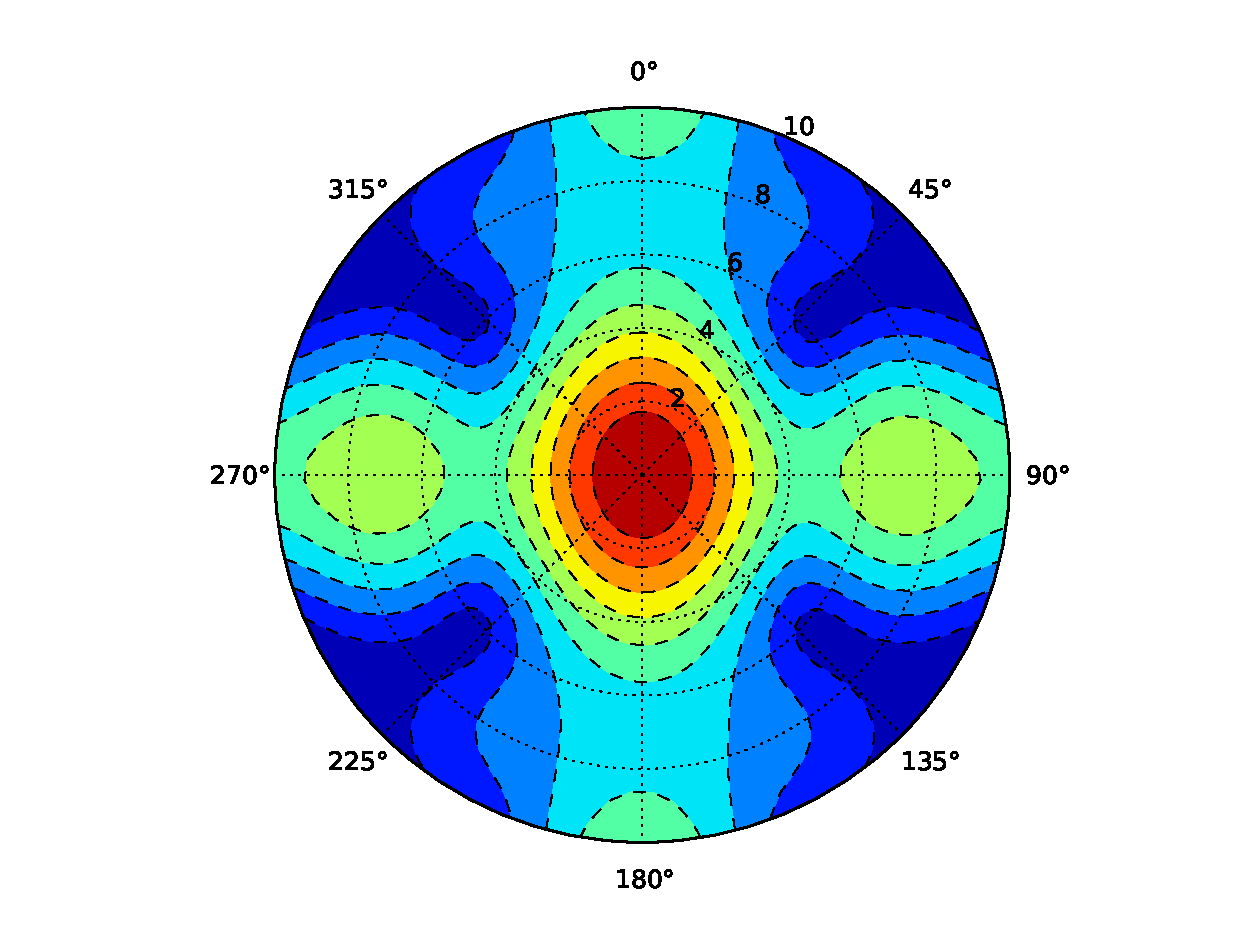
\includegraphics[width=8cm,height=6cm]{fig/chap2/arf_yka_1hz.eps}
}
\hfill{}\subfloat[\label{yka2}]{\centering %
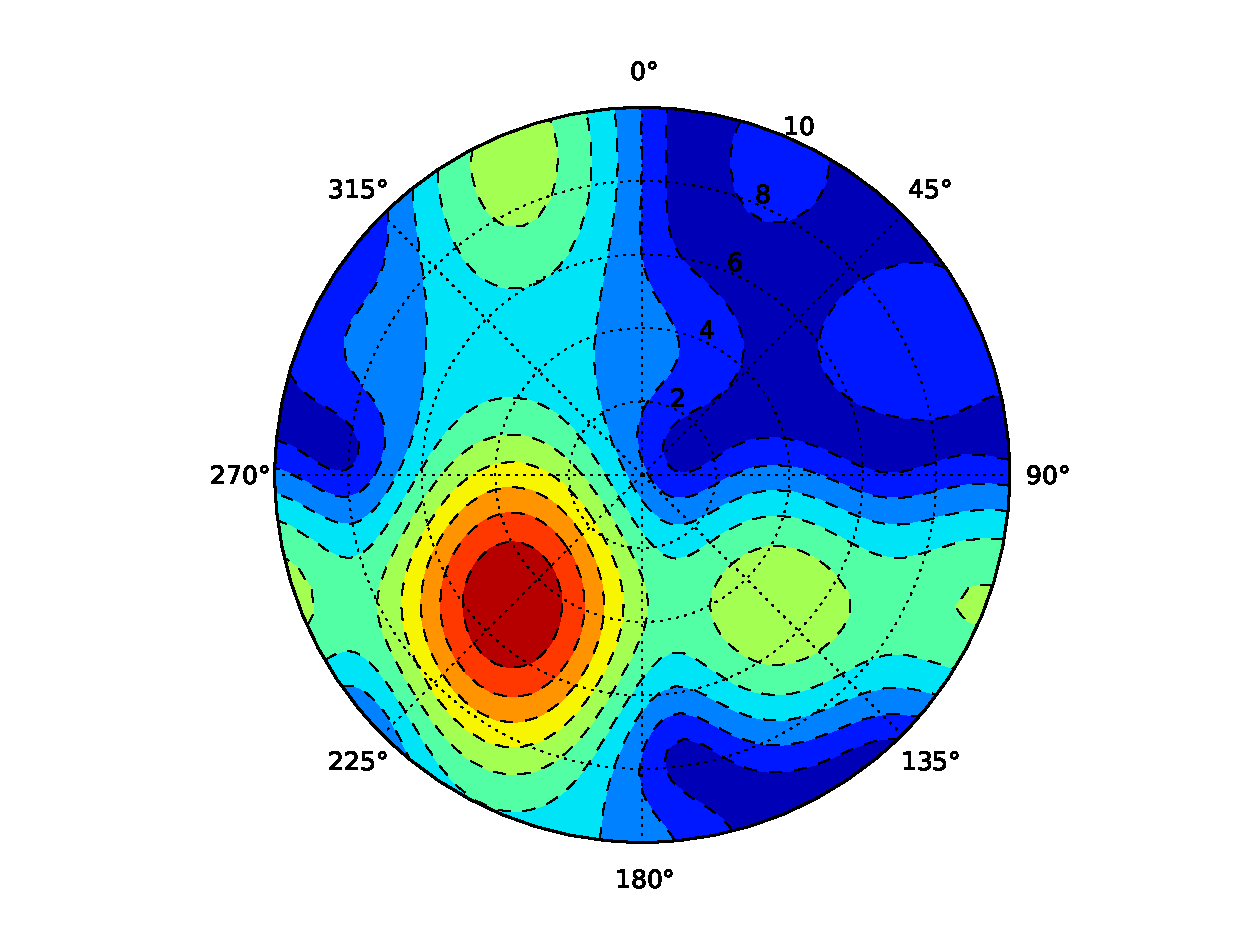
\includegraphics[width=8cm,height=6cm]{fig/chap2/arf_yka_1hz_2.eps}
}
\hfill{}
\caption{YKA台阵的ARF函数(a)$1HZ$的单色平面波从台阵正下方垂直入射的情况。%
(b)慢度$u=5 s/deg$的$1HZ$的单色平面波沿着反方位角$\theta = 225\textdegree$到达台阵的情况。}
\label{yka}
\end{figure}

\begin{figure}[tbph]
\hfill{}\subfloat[\label{grf1}]{\centering %
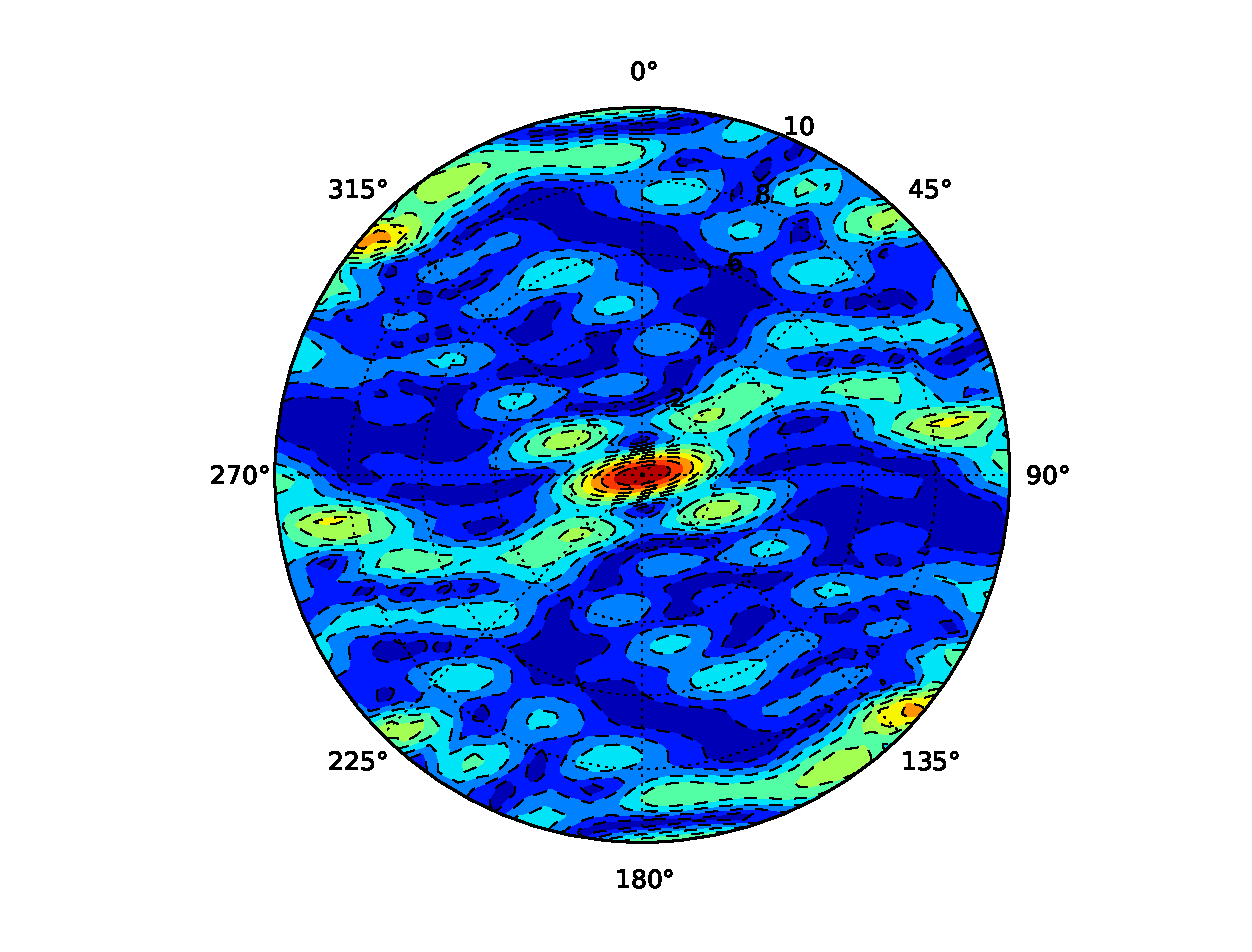
\includegraphics[width=8cm,height=6cm]{fig/chap2/arf_grf_1hz.eps}
}
\hfill{}\subfloat[\label{grf2}]{\centering %
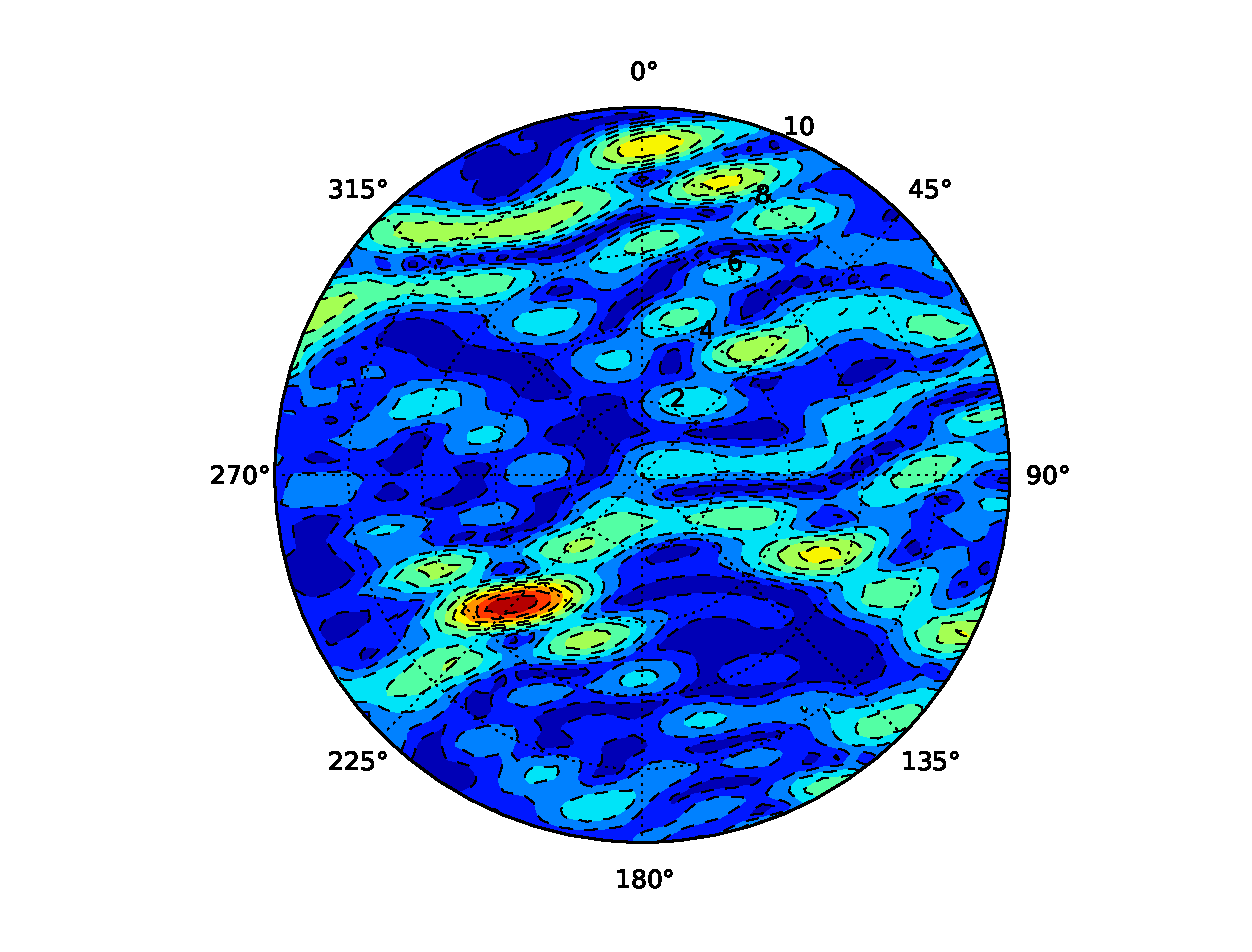
\includegraphics[width=8cm,height=6cm]{fig/chap2/arf_grf_1hz_2.eps}
}
\hfill{}
\caption{GRF台阵的ARF函数(a)$1HZ$的单色平面波从台阵正下方垂直入射的情况。%
(b)慢度$u=5 s/deg$的$1HZ$的单色平面波沿着反方位角$\theta = 225\textdegree$到达台阵的情况。}
\label{grf}
\end{figure}

图\ref{yka}和图\ref{grf}分别表示了YAK和GRF台阵的台阵响应函数(ARF),其中的(a)和(b)
分别对应信号从台阵正下方垂直到达台阵和以$u=5s/deg$的慢度从反方位角$225\textdegree$
到达台阵的情况。可以明显看出小口径的YKA台阵对慢度的分辨能力不佳,ARF函数有很大的主瓣。而
中型口径的GRF台阵慢度分辨率得到了明显提升,主瓣更小。同时由于GRF台阵并不规则,且口径较大,
因此其对来自不同反方位角的信号的分辨能力也不相同。其ARF函数的主瓣并不是呈圆形,而是长轴为
北偏东方向的椭圆,这使得其在北偏东方向上有较高的方位角分辨率,在这个方向上慢度大小分辨率
较低;反之在北西方向慢度分辨率较高,方位角分辨较低。

\subsection{不同频率下的ARF函数}

研究需要关注的不同震相信号其频率不相同,因此需要考察不同频率下台阵响应函数的形态,以此来评估台
阵对某特定频率信号的分辨能力。下面将以YKA、WRA和PSA几个小口径台阵为例子,比较它们在不同频率下的台阵响应函数,台阵的几何形状见图\ref{geometery}。


\begin{figure}[tbph]
\hfill{}
\subfloat[YKA]{%
\centering
\includegraphics[width=4cm,height=3.5cm]{fig/chap2/yka.eps}
}
\hfill{}
\subfloat[WRA]{%
\centering
\includegraphics[width=4cm,height=3.5cm]{fig/chap2/wra.eps}
}
\hfill{}
\subfloat[PSA]{%
\centering
\includegraphics[width=4cm,height=3.5cm]{fig/chap2/psa.eps}
}
\hfill{}
\caption{小台阵YKA、WRA和PSA的几何形状,其中的红色圆圈表示台站的位置。}
\label{geometery}
\end{figure}

三个小口径台阵的口径和台间距均类似,分别为2公里和20公里,只是形态不同。YKA台阵是由两条线状
台阵交叉而成;WRA台阵由从一点出发的两条线状台阵组成,开口向东北方向;PSA台阵则呈现规则的
螺旋形状。图\ref{freq}显示了分别在频率为$1Hz$和$2Hz$情况下,三个台阵的ARF函数。

\begin{figure}[tbph]
\hfill{}
\subfloat[]{%
\centering
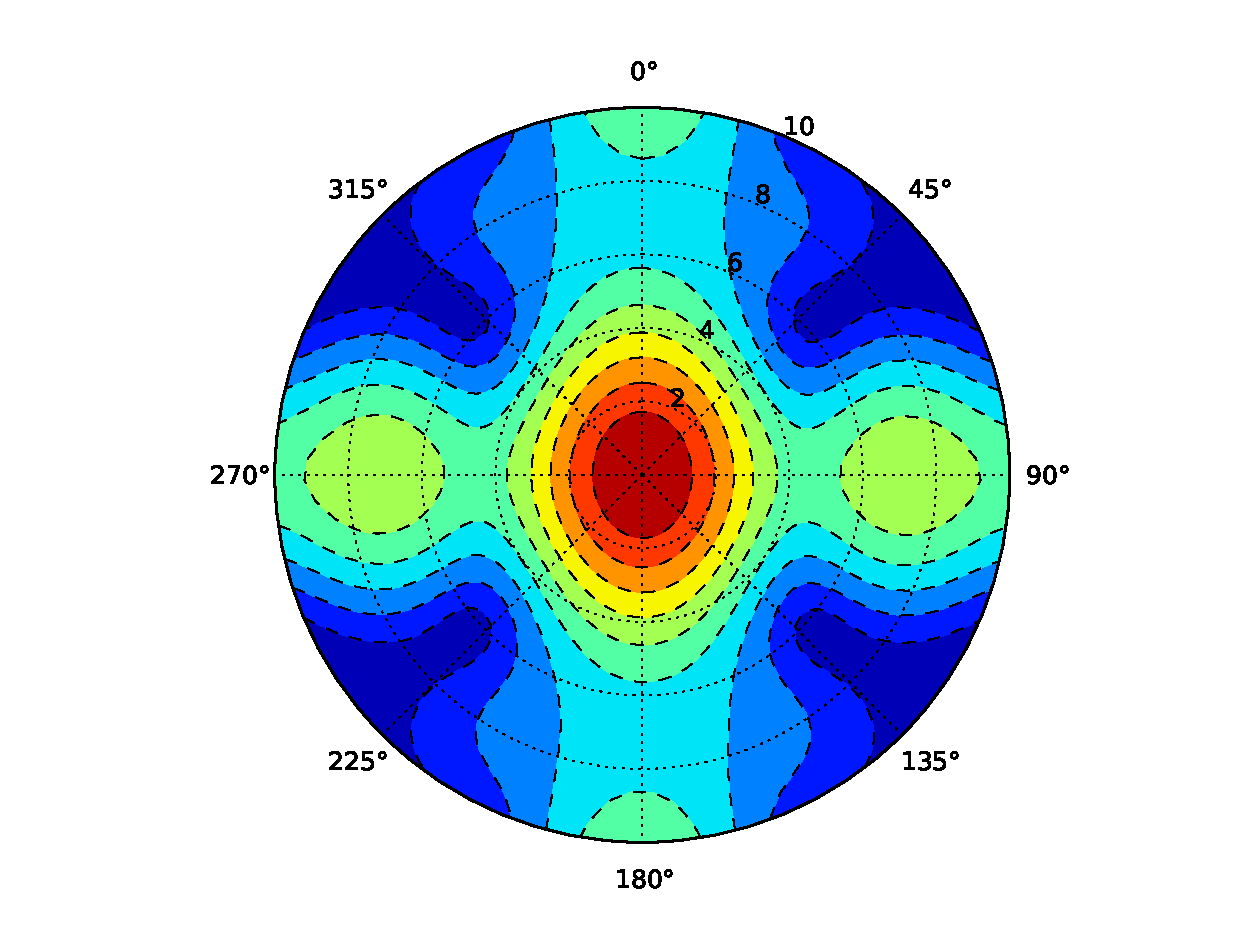
\includegraphics[width=8cm,height=6cm]{fig/chap2/arf_yka_1hz.eps}
}
\hfill{}
\subfloat[]{%
\centering
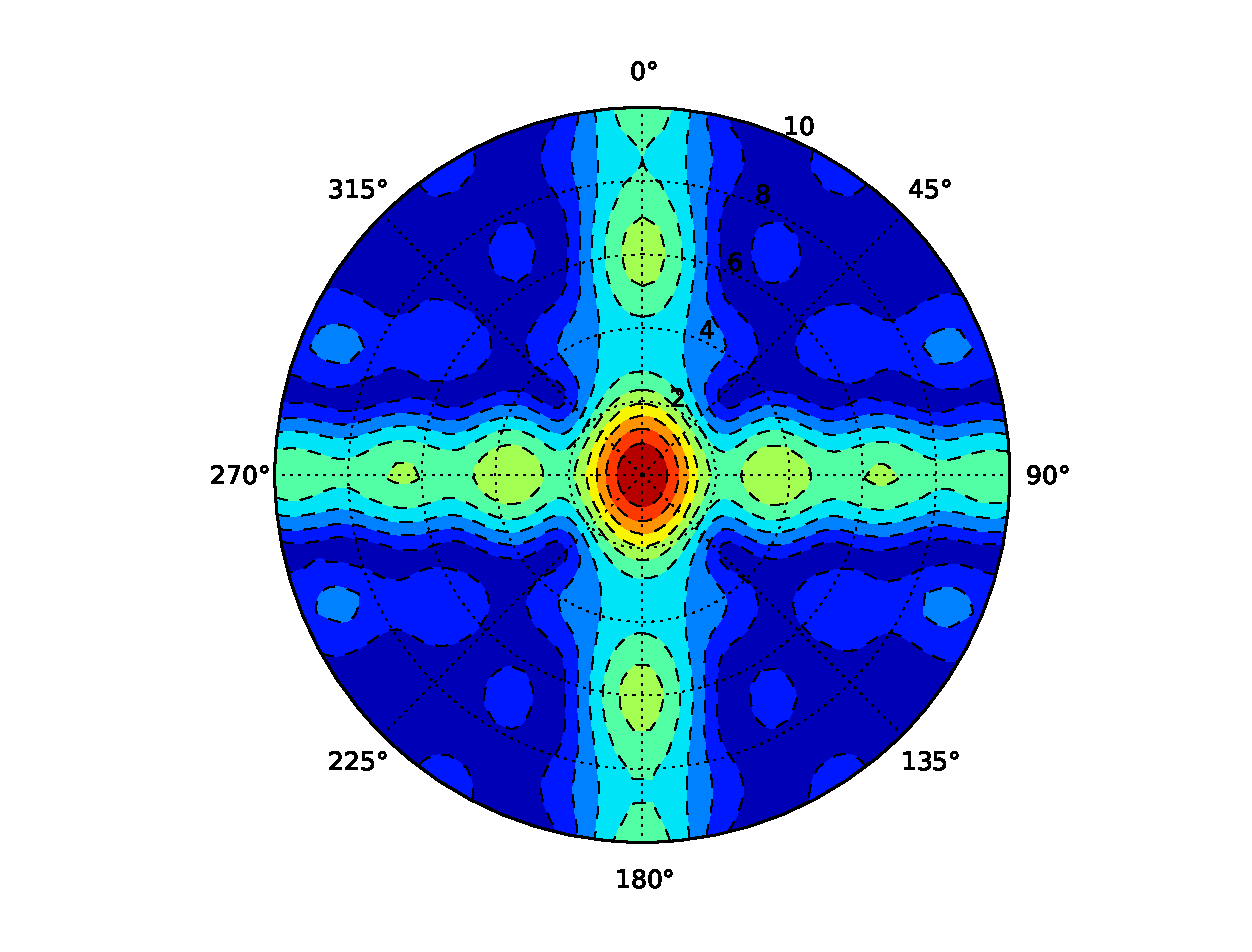
\includegraphics[width=8cm,height=6cm]{fig/chap2/arf_yka_2hz.eps}
}
\hfill{}\\
\hfill{}
\subfloat[]{%
\centering
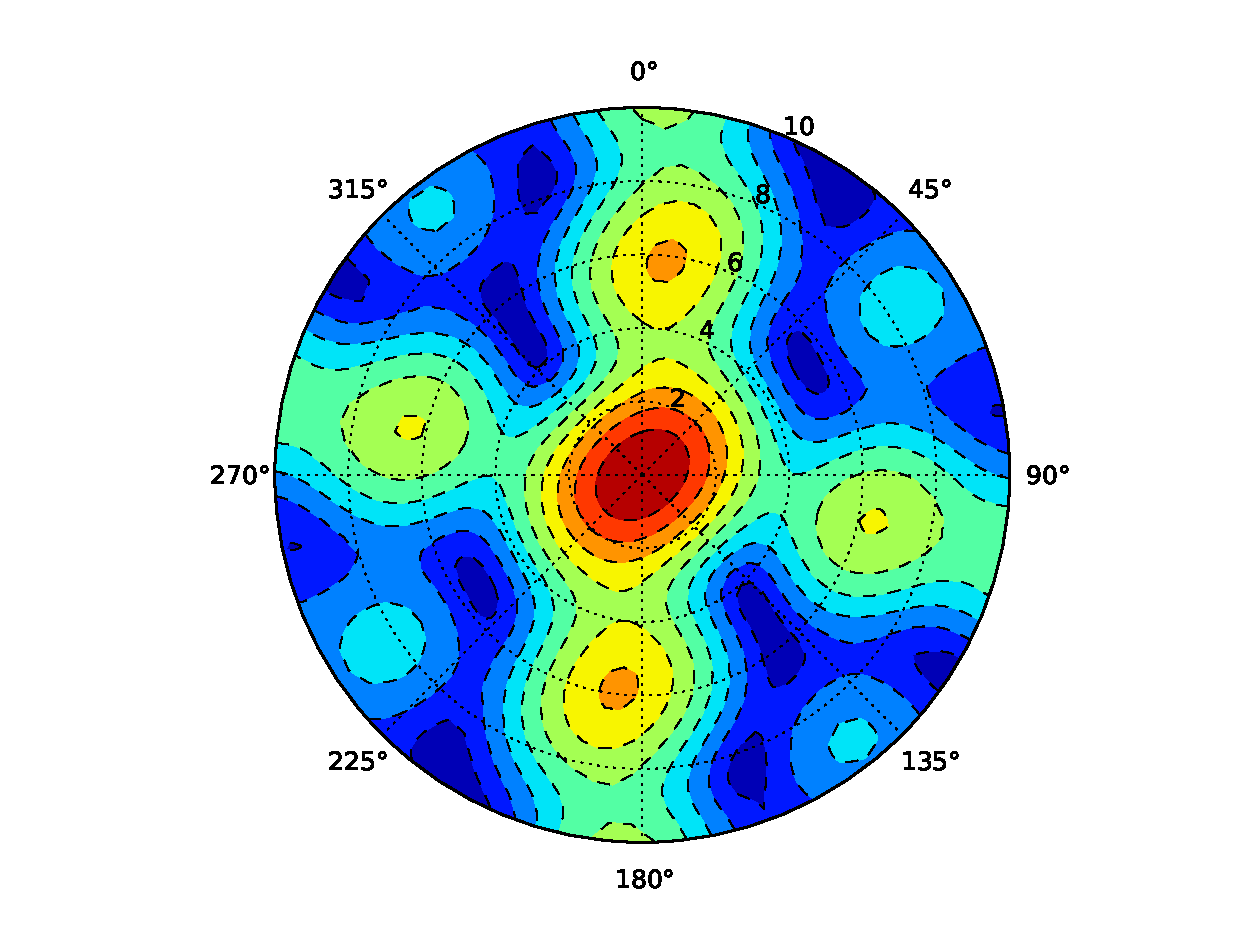
\includegraphics[width=8cm,height=6cm]{fig/chap2/arf_wra_1hz.eps}
}
\hfill{}
\subfloat[]{%
\centering
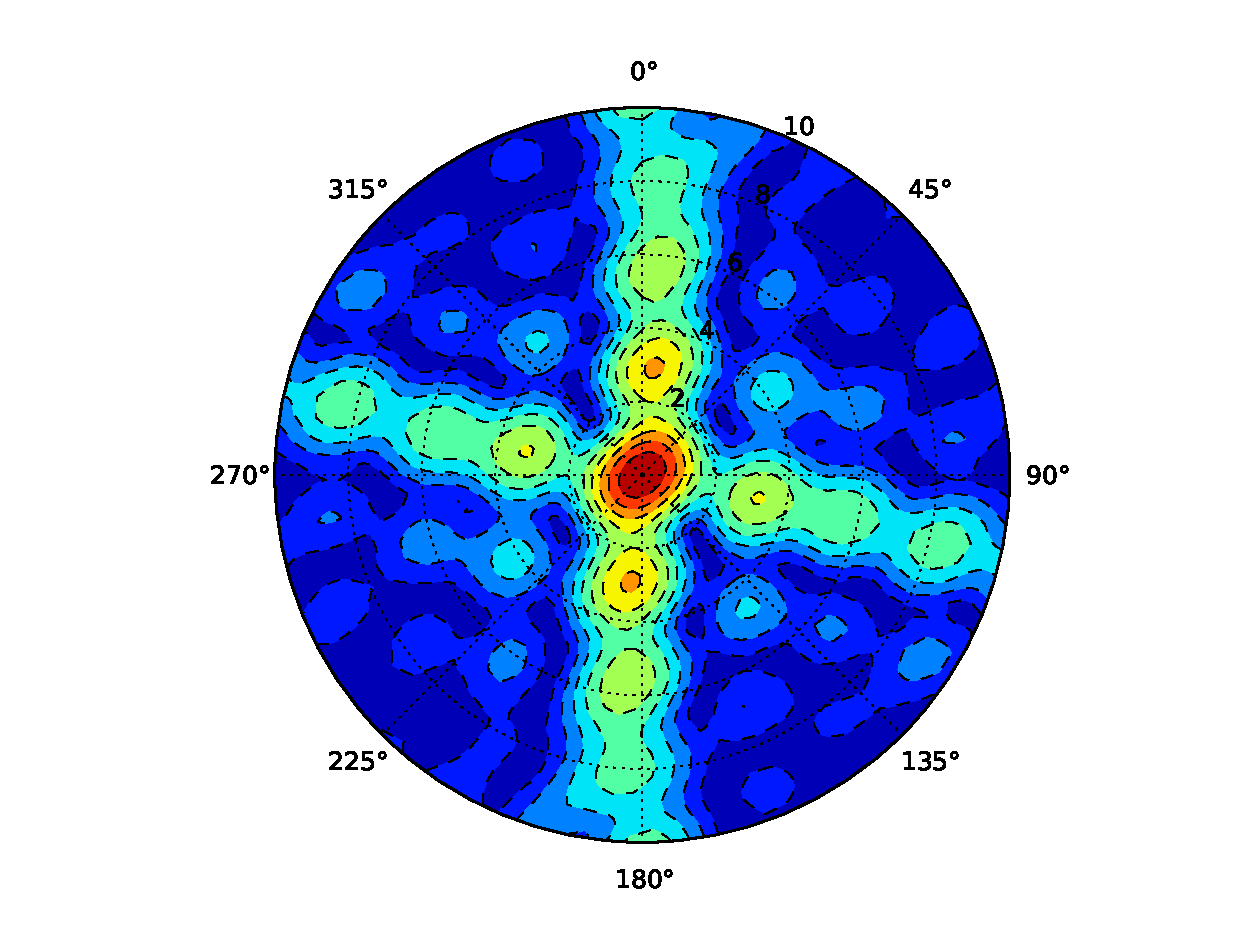
\includegraphics[width=8cm,height=6cm]{fig/chap2/arf_wra_2hz.eps}
}
\hfill{}\\
\hfill{}
\subfloat[]{%
\centering
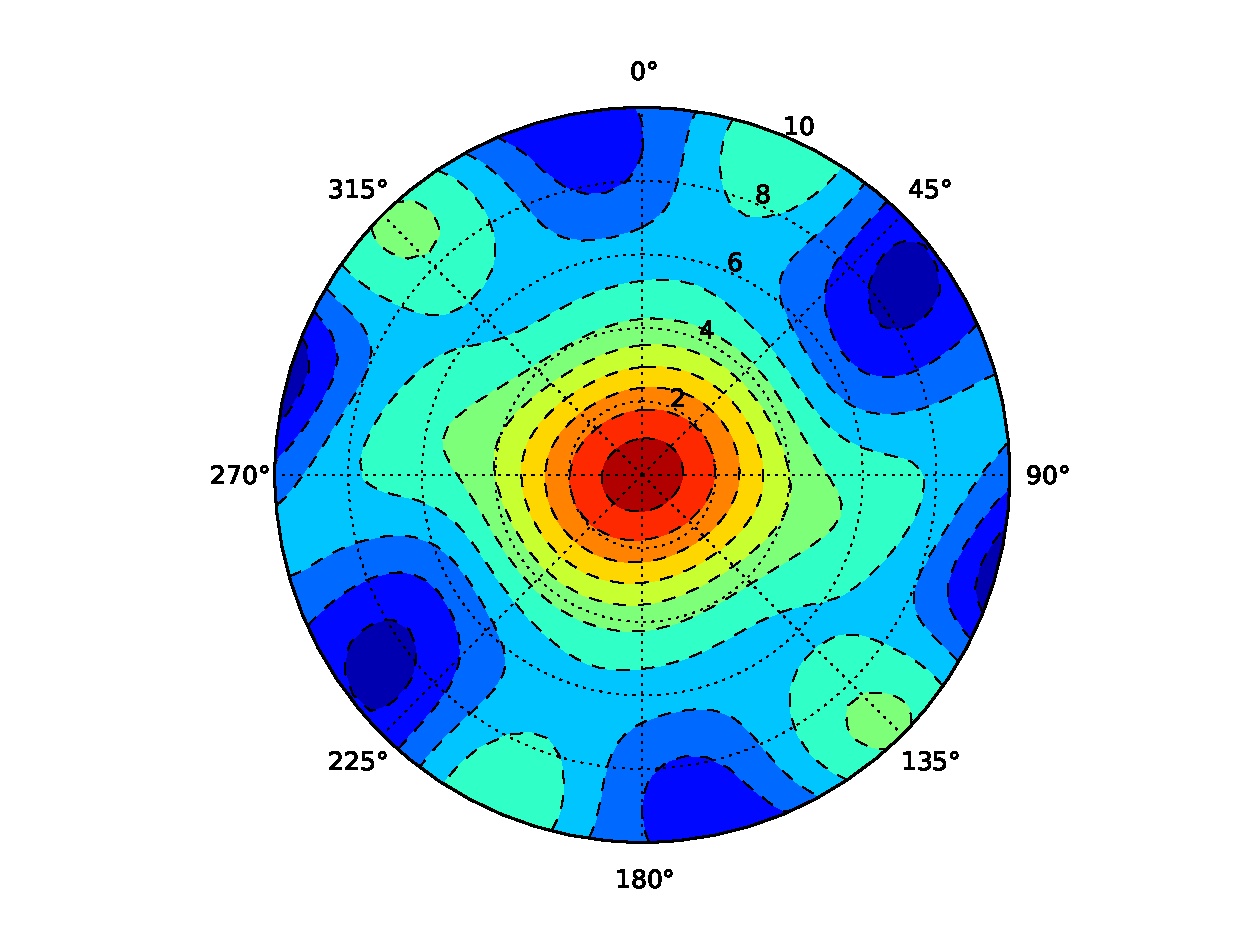
\includegraphics[width=8cm,height=6cm]{fig/chap2/arf_psa_1hz.eps}
}
\hfill{}
\subfloat[]{%
\centering
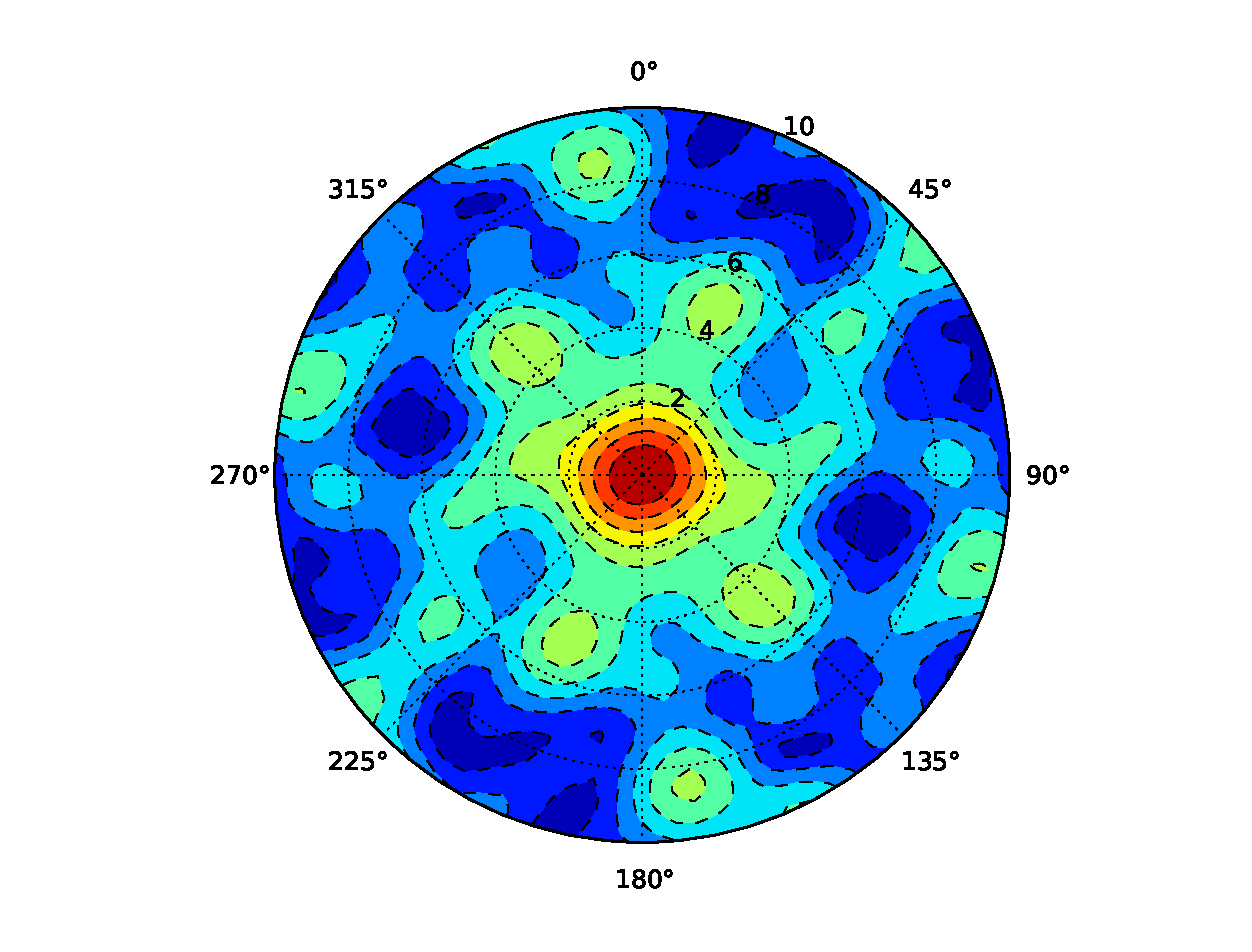
\includegraphics[width=8cm,height=6cm]{fig/chap2/arf_psa_2hz.eps}
}
\hfill{}
\caption{(a)、(b)YKA台阵在1Hz和2Hz下的ARF函数;(c)、(d)WRA台阵在1Hz和2Hz下的ARF函数;%
(e)、(f)PSA台阵在1Hz和2Hz下的ARF函数}
\label{freq}
\end{figure}

图\ref{freq}显示,随着所接收的信号频率增大,台阵乡响应函数的主瓣缩小,变得更加尖锐,对慢度的
分辨力提高,频率$\omega$只起到一个缩放因子的作用;但由于口径均较小,三个台阵对慢度的分辨
能力差异不是很大,ARF函数主要受到口径和台间距影响,台阵几何形状的对ARF函数形态贡献较小。


\section{相位加权叠加(Phased-Weighted Stack)}

PWS方法最早见于地幔间断面转换波的探测\citep{Schimmel1997},能够增强连续的一致信号,压制不连续的随机噪声,目前较为广泛地用于弱信号的识别。典型的例子就有用与前临界PKiKP的研究
\citep{Koper2003,Koper2004},还有用于寻找穿过内核的S波震相PKJKP\citep{Deuss2000}。下面将简要介绍PWS方法的原理还有与Slant叠加的效果对比。

\subsection{PWS方法原理}

PWS是一种非线性叠加方法,它使用一种不依赖振幅的一致性度量方法来加权线性叠加。在叠加的过程中
首先要构建一个解析复信号$S(t)$,它的实部是台站接收到的信号$s(t)$,虚部是则是实部的希尔伯特
变换

\begin{equation}
S(t) = s(t) + i \mathscr{H} [s(t)]
\end{equation}

上式可以写成振幅和相位分离的形式

\begin{equation}
S(t) = A(t) exp[i \Phi (t)]
\end{equation}

其中$A(t)$是地震信号的波包,$\Phi (t)$为瞬时相位。相位叠加的表达式如下

\begin{equation}
c(t) = \frac{1}{N} \left| \sum_{j=1}^{N} exp[i \Phi_j (t)] \right|
\end{equation}

用相位的$\nu$次幂作为加权系数,就得到了PWS的表达式

\begin{equation}
 \nu_{PWS}(t) = \frac{1}{N} \sum_{j=1}^{N} s_j (t)c^{\nu} (t)
\end{equation}

\subsection{PWS与倾斜叠加观测对比}

与简单的线性叠加相比,PWS压制噪声的优势非常明显,能有效突出弱型号。图\ref{compare}
比较了Hi-net~27个台站在PKiKP理论时窗附近的叠加结果,事件位于19.35N,144.76E,震源
深度446.9公里,时间是2010年3月8日。27个台阵位于19.78$\textdegree$至
20.78$\textdegree$的震中距范围内,理论慢度为0.449s/deg,理论到时为942.62s。

\begin{figure}[tbph]
\centering
\subfloat[]{ %
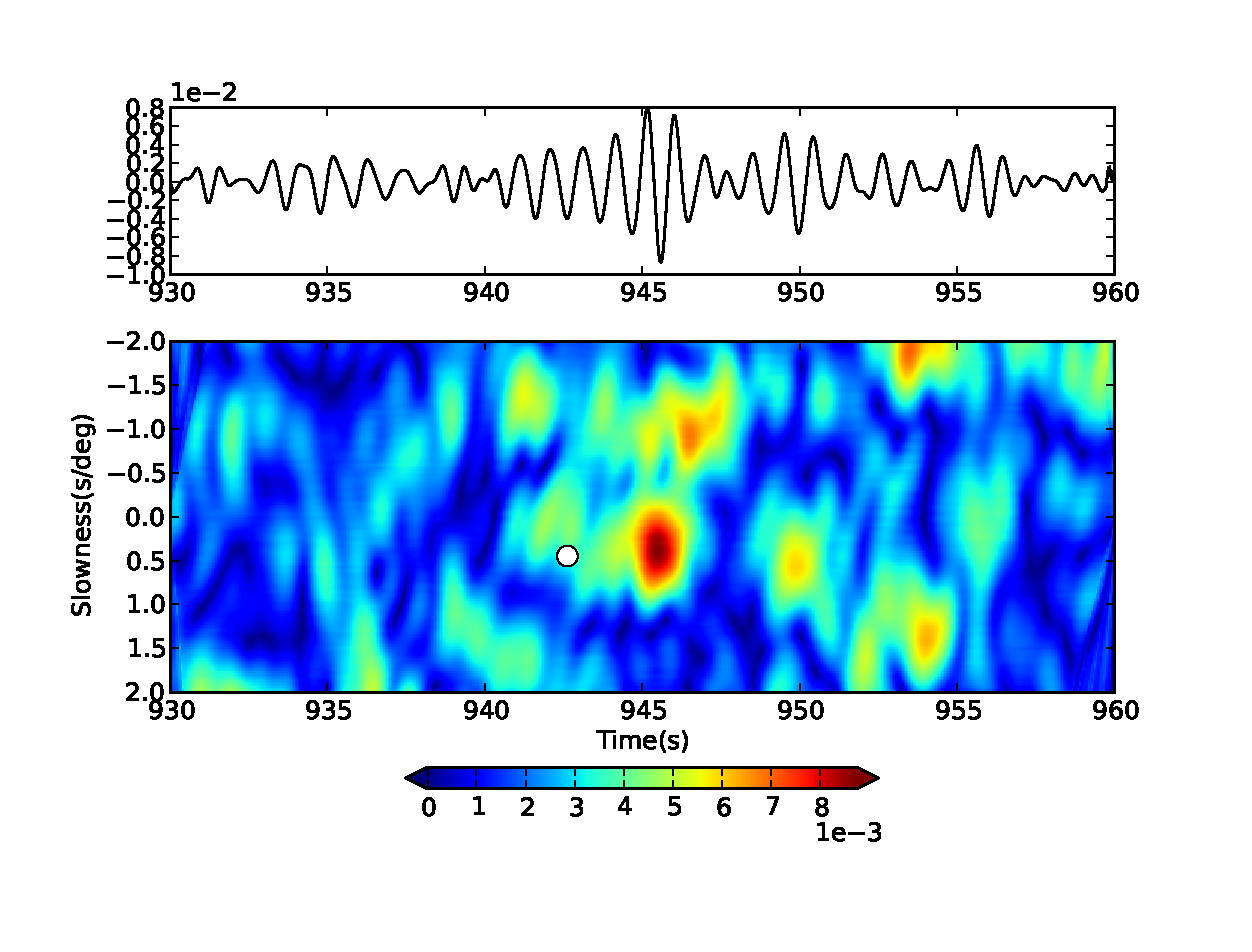
\includegraphics[width=14cm,height=10cm]{fig/chap2/slant_2846275.eps}
}\\
\subfloat[]{ %
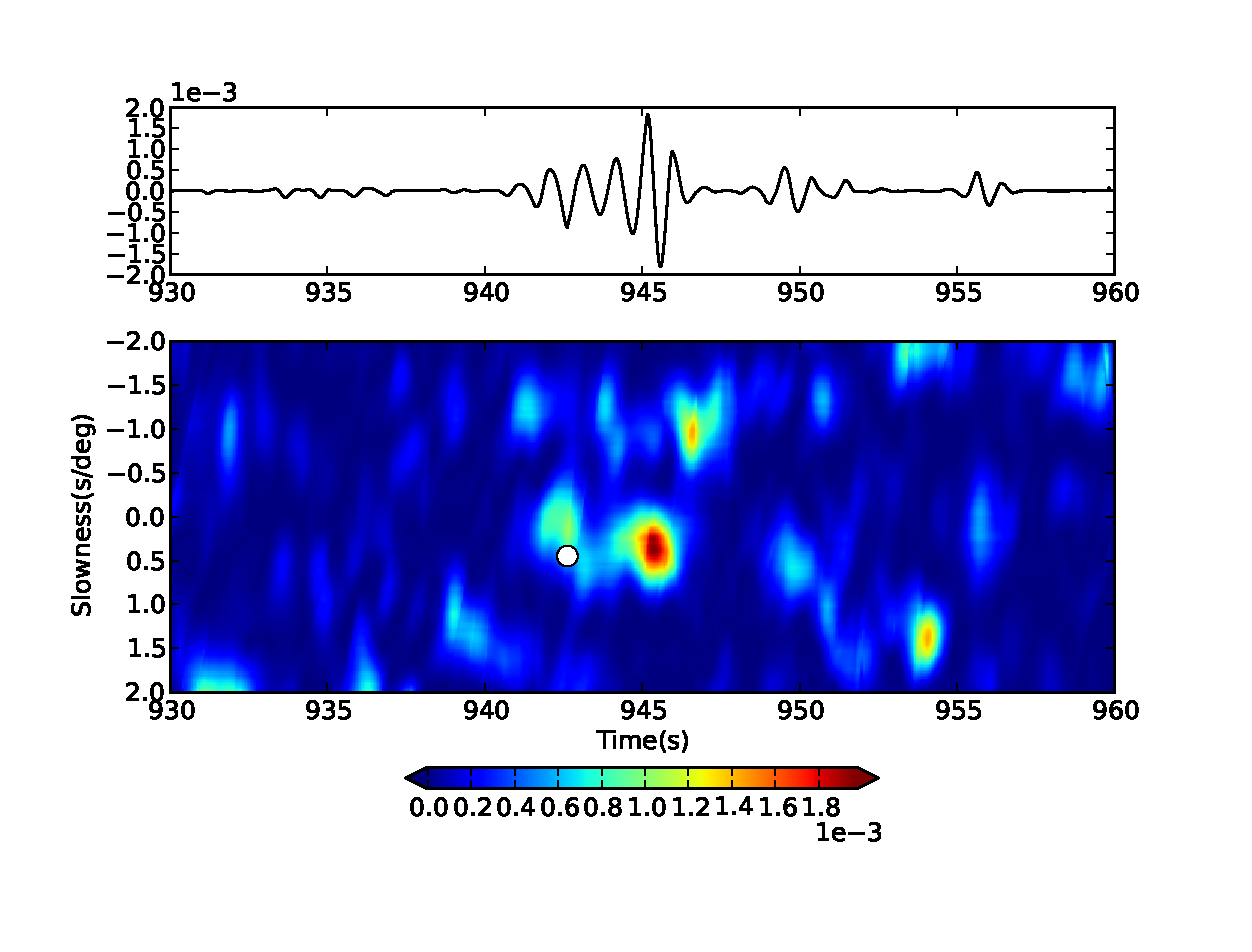
\includegraphics[width=14cm,height=10cm]{fig/chap2/pws_2846275.eps}
}\\
\caption{Slant叠加与PWS的结果对比(a)Slant叠加的结果(b)PWS的结果。上面的部分是叠加最%
大能量出的波形。叠加的慢度搜索间隔是0.02s/deg,白色圆圈表示理论慢度和到时的位置,%
u=0.449s/deg,t=942.62s}
\label{compare}
\end{figure}

可以看出,虽然两种叠加方法得到的最大能量与理论慢度都很接近,但是线性叠加的结果,波包最大能
量处附近还有其他较大的能量区域分布,而PWS则将这些噪声压制得比较干净,从叠加最大能量处的波形看
,PWS的效果也明显更好。图是叠加用到的27道数据,单从波形看,很难分辨出有效信号,在理论到时前后
均有比较大的振幅。

\begin{figure}[tbph]
\centering
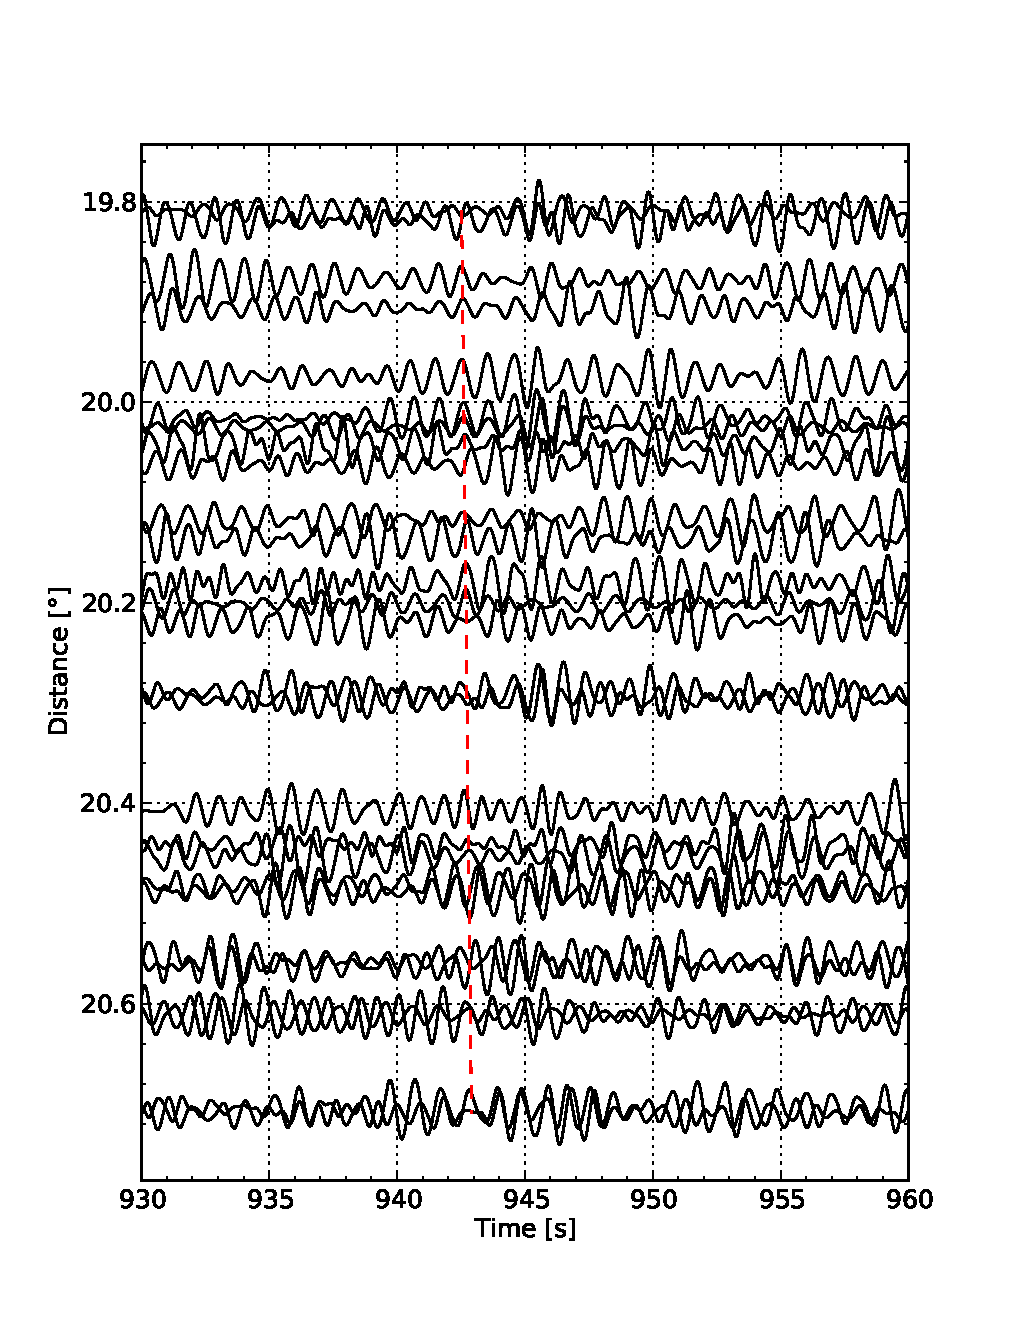
\includegraphics[width=12cm,height=16cm]{fig/chap2/section.eps}
\caption{27道Hi-net台站波形数据,按震中距从小到大排列,其中红色的虚线表示的是PKiKP的理论到时。}
\label{section}
\end{figure}

\begin{figure}
\centering
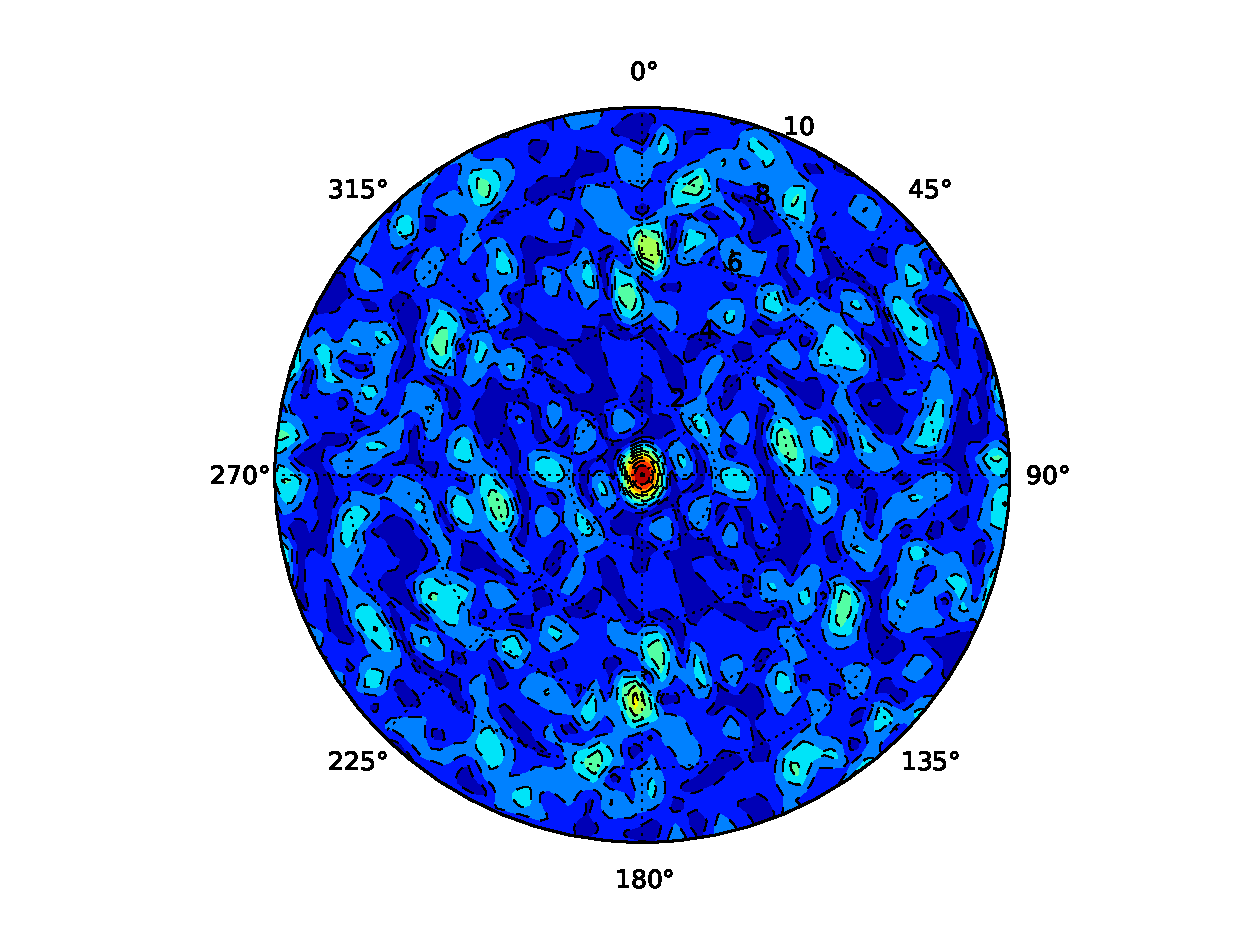
\includegraphics[width=10cm,height=8cm]{fig/chap2/arf_hinet.eps}
\caption{27个台站组成的台阵的ARF函数}
\end{figure}